\section{Introduction}

%-----------------------------------
\begin{frame}

\frametitle{Publications}

% We list below the articles that form the basis of this thesis published by the time of writing:
% TODO: update with your publications

These are the publications (or submissions) that form the basis of this thesis:
\begin{itemize}
%\nobibliography*
    % \item \citet{scassola2025zero} \bibentry{scassola2025zero}.\footnotemark
    % \footnotetext{\scriptsize Code available at: \url{https://github.com/DavideScassola/score-based-constrained-generation}}
    
    % \item \citet{scassola2025graph} \bibentry{scassola2025graph} (Accepted at AAAI$26$)\footnotemark
    % \footnotetext{\scriptsize Code available at: \url{https://github.com/DavideScassola/graph-conditional-flow-matching}}
    
    % \item \cite{bortolussi2023model} \bibentry{bortolussi2023model}.

    % \item \cite{cornalba2024multi} \bibentry{cornalba2024multi}.
    \item \textbf{Zero-Shot Conditioning of Score-Based Diffusion Models by Neuro-Symbolic Constraints}. Scassola, D., S. Saccani, G. Carbone, and L. Bortolussi. \textcolor{blue}{Accepted at AAAI 2025}.
    
    \item \textbf{Graph-Conditional Flow Matching for Relational Data Generation}. Scassola, Davide, Sebastiano Saccani, and Luca Bortolussi. \textcolor{blue}{Accepted at AAAI 2026}.    
    
    \item \textbf{A Sobering Look at Tabular Data Generation with Probabilistic Circuits}. Scassola, D., Ponsford D., et al. \textcolor{blue}{Submitted to UAI 2026}.
    
\end{itemize}

Other publications:
\small
\begin{itemize}
    \item \textit{"Model Abstraction and Conditional Sampling with Score-Based Diffusion Models."} Bortolussi, Luca, et al. International Conference on Quantitative Evaluation of Systems (2023).
    \item \textit{"Multi-objective reward generalization: improving performance of Deep Reinforcement Learning for applications in single-asset trading."} Cornalba, Federico, et al. Neural Computing and Applications (2024).
\end{itemize}


%We will highlight when a chapter or (sub)section of a chapter is based on a published work.
%
% TODO: update with your publications

% The following other publications during the PhD studies do not contribute to the contents of this thesis: \citet{bortolussi2023model}, a short paper discussing a potential way to apply conditional sampling with score-based generative models to surrogate stochastic models, and \citet{cornalba2024multi}, where we investigate the potential of Multi-Objective, Deep Reinforcement Learning for stock and cryptocurrency single-asset trading.
\end{frame}
%-----------------------------------




%-----------------------------------
\begin{frame}

\frametitle{Context}

\begin{itemize}
    \item Generative modeling has advanced rapidly, its development mostly focused on unstructured data as images, videos, audios and text.
    \item \textbf{Tabular data generation} is less popular despite its practical importance (financial transactions, patient records, commercial databases, etc)
    \item Tabular data is structured data organized in rows and columns, where each row is an observation and each column is a feature or attribute.
    \bigskip
    % Please add the following required packages to your document preamble:
% \usepackage{booktabs}
\begin{table}[]
\small
\begin{tabular}{@{}llllll@{}}
\toprule
\textbf{age} & \textbf{education} & \textbf{sex} & \textbf{capital-gain} & \textbf{native-country} & \textbf{income}   \\ \midrule
39           & Bachelors          & Male         & 2174                  & United-States           & \textless{}=50K   \\
50           & Bachelors          & Male         & 0                     & Jamaica                 & \textless{}=50K   \\
%38           & HS-grad            & Female       & 0                     & United-States           & \textgreater{}50K \\
%53           & 11th               & Male         & 5178                  & Cuba                    & \textgreater{}50K \\
37           & Masters            & Female       & 14084                 & United-States           & \textgreater{}50K   \\
$\dots$      & $\dots$            & $\dots$      & $\dots$               & $\dots$                 & $\dots$           \\ \bottomrule
\end{tabular}
\end{table}
    \bigskip
    %\item Tabular data is ubiquitous in real-world systems: financial transactions, patient records, commercial databases, etc.
    %\item Key applications of tabular data generation: privacy preservation, data augmentation, probabilistic inference, anomaly detection.
\end{itemize}



\end{frame}
%-----------------------------------


%-----------------------------------
\begin{frame}

\frametitle{Applications of Tabular Data Generation}
\begin{itemize}
    \item \textbf{Privacy preservation}: share synthetic data that mimics the statistical properties of real data without revealing sensitive information.
    \item \textbf{Data augmentation}: create additional training data to improve the performance of machine learning models, especially in cases of class imbalance or limited data availability.
    \item \textbf{Probabilistic inference}: perform probabilistic reasoning on the generated data, e.g., computing probabilities (anomaly detection).
\end{itemize}

\begin{center}
    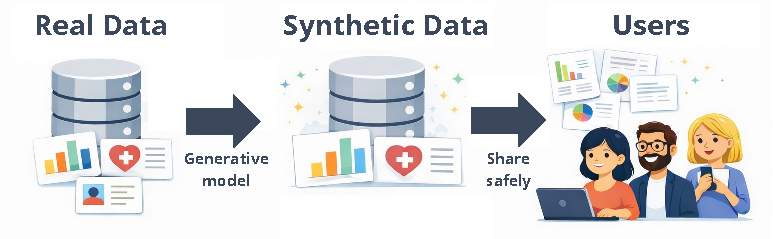
\includegraphics[width=0.7\textwidth]{assets/images/synthetic_data_infographic.pdf}
\end{center}

\end{frame}
%-----------------------------------


%-----------------------------------
\begin{frame}

\frametitle{Challenges of Tabular Data Generation}

\begin{itemize}
    \item \textbf{Complex distributions}: multimodality, heavy tails, inflated values
    \item \textbf{Intricate dependencies}: nonlinear, high-order, non-monotonic relationships
    \item \textbf{Heterogeneous data types}: continuous, ordinal, categorical, binary, temporal
    \item \textbf{Missing data}: cannot be trivially imputed
    \item \textbf{Hard constraints}: physical, logical, or business rules
    \item \textbf{Quality evaluation}: difficult to assess compared to images or text
    \item \textbf{Privacy concerns}: avoid leaking sensitive information
    \item \textbf{Relational data}: complex dependencies across multiple interconnected tables
\end{itemize}

\end{frame}
%-----------------------------------


%-----------------------------------
\begin{frame}
\frametitle{Limitations of Current Techniques}

Despite significant progress, several limitations remain, especially regarding flexibility:

\begin{itemize}
    \item \textbf{Constraints}: Many models cannot efficiently incorporate user-specified constraints in the generated data (known facts, partial observations, logical rules). %Most existing methods require retraining or fine-tuning the model for each new constraint.
    \item \textbf{Relational data}: Current approaches for relational data generation cannot generate any type of relational dataset, or are not expressive enough to model complex inter-table dependencies.
    \item \textbf{Probabilistic queries}: General probabilistic queries are generally not possible with most state-of-the-art models for tabular data generation: density computation, marginalization, inference under missing data, etc.
\end{itemize}

\end{frame}
%------------------------------------

%-----------------------------------
\begin{frame}

\frametitle{Contribution}

\textbf{Research Questions:}
\begin{itemize}
    \item \textbf{Q1}: Can we generate data from a pre-trained diffusion model while enforcing arbitrary user-defined logical constraints?
    \item \textbf{Q2}: Can we design expressive generative models capable of generating relational data with complex structural dependencies without any implicit independence assumptions?
    \item \textbf{Q3}: Can we train tractable yet expressive generative models for tabular data?
\end{itemize}

\bigskip

\textbf{Contributions:}
\begin{enumerate}
    \item Method for conditional sampling from Score-based Diffusion Models under logical constraints
    \item Flow-matching framework for relational databases with arbitrary structures
    \item Analysis of probabilistic circuits as tractable generative models
\end{enumerate}

\end{frame}
%-----------------------------------